\chapter{Literature Review} \label{chap:ch2}

This chapter reviews the current literature on graph-based time series forecasting techniques. In addition, it focuses on the relationship between Graph Neural Networks (GNN), architectures, and temporal modeling techniques.

Owing to the large volume of new work being developed in the field and the variety of ways in which researchers have approached the problem of forecasting time series using graphs, this literature review is organized into clearly defined architectural and methodological categories.


\section{Background: Graph Neural Networks for Time Series Forecasting}

Jin et al.'s ~\cite{jin2024survey} recent survey on GNNs for time series analysis is used as a basis for organizing this literature review. The survey presents a comprehensive categorization of GNN methodologies applied to time series data across four broad tasks: forecasting, classification, imputation, and anomaly detection. Additionally, Jin et al. organized all previous methods along three axes: graph construction strategies, temporal modeling components, and learning objectives.

Furthermore, Jin et al. highlighted that time series forecasting has been one of the most heavily studied application domains for GNNs and that many of the applications fall under the category of spatiotemporal forecasting domains, such as traffic forecasting and energy consumption prediction. For example, most GNN models used for time series forecasting use a similar paradigm: relational dependencies are modeled using a graph-based message-passing mechanism, and temporal dependencies are modeled using some form of recurrent, convolutional, or attention mechanisms.

Thus, Jin et al.’s survey provides a useful reference framework for understanding how the architectures of graph-based models are currently designed and evaluated and for identifying the foundational models, architectures, and open problems that relate to the specific research questions addressed within this dissertation.
\subsection{Embedding Decoupled Graph Representations} \label{sec:decoupled_embeddings}

While spatio-temporally coupled end-to-end GNN's update the node representations on-the-fly while making predictions, another way to represent graphs is to separate the structural representation of a graph from its temporal representation. For example, the relational structure of a graph is first mapped to a lower-dimensional space using some form of unsupervised learning. These static nodes or graph embeddings are then used as exogenous spatial information in a separate temporal forecasting model.

One key example of this type of methodology is \textit{\textbf{Graph2Vec}} ~\cite{narayanan2017graph2vec}, which uses techniques similar to those found in neural document embedding to learn task-agnostic and distributed representations of arbitrarily sized graphs. While Graph2Vec treats a graph as a “document” and its root sub-graphs as “words,” it learns embeddings using a skip-gram architecture without any supervision. Using this technique allows us to overcome the limitation of traditional handcrafted graph kernel functions when attempting to capture the complexity of a graph topology via nonlinear substructure sampling.

In the context of multivariate time series forecasting, decoupled methodologies such as Graph2Vec (as well as its node-level variant Node2Vec\cite{DBLP:journals/corr/GroverL16}) provide important methodological baseline comparisons. Because the graph embeddings are created before any forecasts, they are used as pre-computed relational prior. These static vectors can be concatenated with historical time-series data and fed into traditional temporal architectures, such as LSTMs or MLPs. In contrast to fully joint pipelines, where graph learning and temporal forecasting occur simultaneously, the decoupled pipeline provides both computational efficiencies owing to reduced memory/computational overheads for training the temporal model and task-agnostic learned embeddings, as they are not biased towards a specific forecast horizon/temporal loss function. However, significant trade-offs are associated with decoupling. Due to their independence from the forecasting objectives, they will not be able to adapt to changing temporal relationships or error signals during training. The embeddings remain fixed and do not have the inductive ability of models that learn spatial message passing and temporal updates in conjunction with them.

The fundamental evaluation question of this dissertation is how to compare fixed task-agnostic embeddings (that is, Graph2Vec) to the dynamic, end-to-end representations learned by inductive GNN architectures (for example, graph convolutional networks (GCNs)). A comparative analysis between these two paradigms will help determine whether the increased computation required for integrated message passing results in improved predictive performance in real-world retail environments.

\subsection{Spatiotemporal GNN Architectures} \label{sec:stgnn}

The first type of architecture for GNN’s that was developed was based on spatiotemporal GNN's. They are also referred to as Multivariate Time-Series Forecasting Models. The purpose of the GNN approach is to develop a model that can consider both the spatial (location) and temporal (time) dependencies found in the data. These types of problems often occur when attempting to forecast values at locations on a grid, such as weather stations, power substations, and traffic cameras. Using GNN's, a graph structure that captures the spatial relationships between locations can be created and then used to determine the temporal relationships.

One common design pattern for ST-GNN's is to separate the processing of spatial relationships from the processing of temporal relationships. To process spatial relationships, we performed some form of graph convolution operation or message passing. Once we have processed the spatial relationships, we would pass the results to a temporal processing unit (such as RNN, TCN, or Attention Mechanism). The temporal unit then processes the temporal aspects of the data.

Many early examples of ST-GNN's used predefined spatial structures. For example, DCRNN~\parencite{li2018dcrnn} uses diffusion-based graph convolutions combined with gated recurrent units to model traffic flow dynamics. The DCRNN processes the spatial relationships between neighboring nodes in a sequential manner and then performs temporal forecasting. A similar type of model, STGCN~\parencite{yu2018stgcn}, uses graph convolutions to process spatial relationships and one-dimensional convolutions along the time dimension to process temporal relationships.

Later studies built upon these earlier studies but improved them by using more powerful and/or efficient temporal processing units. An example of this is the Graph WaveNet~\parencite{wu2019graphwavenetdeepspatialtemporal}. Graph WaveNet replaced RNN’s with Temporal Convolution Networks (TCNs) allowing for more parallelized computation and better multi-horizon forecasting capabilities. Although Graph WaveNet includes an adaptive graph learning module that allows for flexibility in the selection of the adjacency matrix, it still adheres to the basic spatiotemporal premise that forecasting is driven by spatial message passing followed by temporal modeling.

While successful in certain areas of study, such as traffic and energy consumption forecasting, there are many limitations to traditional ST-GNN forecasting models. One limitation is that their heavy reliance on an explicit spatial structure limits their potential application in all other areas where relationships exist but do not exist geographically (semantic, latent, contextual, etc.). Another limitation is that most ST-GNN models assume a static or slow-changing graph structure, which greatly hinders their capability to learn about rapidly changing and dynamic interactions. Finally, ST-GNN models generally only measure performance based on downstream forecasting accuracy without providing any insights into whether the topology of the learned graph representation is stable or interpretable.

According to Jin et al.~\parencite{jin2024survey}, these limitations suggest that the underlying assumptions and design decisions made regarding ST-GNN’s may not necessarily apply to other non-spatial domains. Therefore, developing generalized GNN-based methods has become increasingly important, particularly in multivariate forecasting scenarios, where the graph is either learned or latent.

\subsection{Multivariate Time Series Forecasting with Learned Graphs} \label{sec:mts_learned_graphs}

In addition to the previously discussed methods, several other models have recently been proposed that focus on multivariate time-series forecasting problems without predefined graph structures. 

These models represent each node in the graph as a variable or element in a multivariate time series. 

Therefore, instead of being defined a priori based on the physical or spatial location of entities, the underlying graph structure is determined automatically from the data. These approaches were explicitly designed to address domains where establishing a ground-truth topology is either impossible or methodologically flawed, establishing a strong academic precedent for relying entirely on latent structural inference."

This type of representation can capture implicit semantic, functional, or latent relationships among different elements of a time series.

One of these approaches is the Multivariate Time Series Graph Neural Network \ac{MTGNN} ~\cite{wu2020connectingdotsmultivariatetime}, which uses a learnable adjacency matrix to express inter-variable dependencies via trainable node embeddings. 

Both types of parameters are learned simultaneously with respect to the forecasting objectives. 

Using this feature, the MTGNN model can identify latent relationships between the time-series elements. 

Subsequently, the model applies graph convolutional layers to the variables to propagate information among them. 

Finally, after applying both convolutional and recurrent components for temporal prediction, the model performs time-series forecasting. 

Thus, this design allows the MTGNN to extend its applicability beyond spatiotemporal domains and to general multivariate forecasting problems.


\begin{figure}[htbp]
    \centering
    \includegraphics[width=0.5\linewidth]{figures/mtgnnarchiteture.png}
    \caption{ The graph-evolution module, demonstrating the flow from temporal sequence inputs to the dynamic generation of the adjacency matrix. The integration of temporal convolutions with a linear layer allows for the continuous structural adaptation of $A$. Source \cite{wu2020connectingdotsmultivariatetime}}
    \label{fig:mtgnn}
\end{figure}

Another similar method is the Adaptive Graph Convolutional Recurrent Network (\ac{AGCRN})~\cite{bai2020adaptivegraphconvolutionalrecurrent}. 

Unlike MTGNN, AGCRN dynamically generates an adjacency matrix at each step of the training process. 

Each node in the network has a unique learnable vector (node embedding). 

An edge exists between two nodes if there is a high degree of similarity between the corresponding node embeddings. 

With this adaptive mechanism, the \ac{AGCRN} can create an optimal adjacency matrix during the training phase. 

Additionally, the AGCRN utilizes RNNs to incorporate temporal dependence into the forecast while modeling relationship structures. 

By removing the constraints imposed by predefined domain knowledge regarding graph construction, the AGCRN establishes a flexible platform for representing changes in interdependencies within multivariate time-series data. Crucially, both MTGNN and AGCRN establish an important academic precedent because they were explicitly designed for datasets that fundamentally lack a predefined ground-truth topology. In these frameworks, the absence of a fixed relational map is not viewed as a limitation of the data but rather as the primary methodological motivation for relying entirely on latent structural inference.

Finally, the Graph for Time Series (GTS) framework ~\cite{shang2021discretegraphstructurelearning} further develops this trend by formulating graph learning as a structural inference task. 

GTS uses probabilistic reasoning to infer latent graph structures. 

It draws conceptual similarities from Neural Relational Inference Models. 

However, unlike many contemporary continuous adjacency matrix learning techniques, GTS focuses on discrete/interpretable relational structures and clearly separates the tasks of learning graph structures and predicting the future values of time series. 

Because GTS provides clear insights into the contributions of learned relations to forecasting performance and enables the assessment of the relevance of graph quality for subsequent forecasting tasks, it constitutes an important advancement in this field.

Together, these studies illustrate a shift from using predetermined graph structures in specific domains to employing graph learning to identify relational structures from observed data to predict the future values of multivariate time series. 

Furthermore, by providing direct learning of relational structures from data and enabling predictions in cases with multiple complex non-spatial and context-dependent relationships among variables, this trend has significant implications for applications such as retail demand forecasting. 

For example, in retail demand forecasting, relationships exist among products owing to substitution effects, complementarity, promotional events, and/or common customer behavior rather than physical location.

Although flexible and capable of modeling relationships between variables that were not easily accessible to previous time series forecasting methods, learned-graph forecasting methods have introduced several additional challenges. 

First, adjacency matrices constructed via learned graph mechanisms tend to be dense and are therefore difficult to understand. 

Second, although adjacency matrices are typically considered important for determining forecasting accuracy and quality, they are rarely assessed independently. 

Finally, when dealing with larger numbers of variables, scalable graph learning becomes increasingly challenging because most currently available graph learning techniques require a quadratic increase in computation relative to the number of nodes in the graph.

Therefore, because learned-graph multivariate forecasting models provide a critical link between GNN architectures developed for spatiotemporal forecasting and application domains characterized by semantic relationships, this link serves as a basis for the research questions investigated in this thesis and motivates research directed toward developing appropriate graph-based representations for use in retail forecasting.



\section{Process for Systematic Review}

There has been a large increase in the number of studies related to multivariate time series forecasting in recent years, especially because of the development of models that specifically consider the interdependencies among variables, hidden relational structure of data, and learned representations of graphs. There are multiple areas of focus within these different types of research (including graph construction, structural learning, relational embedding, and time-series representation learning). Given the breadth and interdisciplinarity of this body of work, a systematic literature review was conducted to identify, organize, and analyze relevant contributions in a structured and reproducible manner.

The objective of this review is to identify methods that learn or infer relational structures from time-series data and/or  learn time-series representations that explicitly capture latent dependencies among variables, particularly in the context of forecasting. To this end, a systematic review methodology was adopted that included an identification phase, followed by screening and an eligibility assessment. The overall workflow followed the PRISMA-style guidelines, with a clear separation between record identification, deduplication, screening, and final inclusion.

\subsection{Identification Phase}

The authors identified possible literature by searching three prominent digital libraries: the ACM Digital Library, IEEE Xplore, and Scopus. The selection of these libraries was based on the fact that they contain an extensive collection of scholarly research, including peer-reviewed journals and conferences in the areas of computer science, machine learning, and data mining. To provide as complete a literature search as possible, the authors developed two query strings. Each string was used to identify different, yet related, themes in the literature. A third query string was also created to include studies focused specifically on retail sales forecasting, where graph neural networks and/or graph-based learning techniques were used on a product-level multivariate time series to model inter-product dependency relationships to enhance future sales/demand predictions. This final query was added because the authors' dataset contained only historical sales information, product hierarchy (department/category), and promotional signals; therefore, the authors did not have access to any customer behavior data (baskets, sessions, clicks, etc.) and needed to find forecasts in alignment with item/store-level sales predictions and exclude any recommender system-focused literature.

The first query focused on the literature that explicitly addressed graph construction/structure learning for time-series forecasting. The second query focused on time-series representation learning methods that learn latent relationship structures and dependencies.

\paragraph{Query 1 (Graph-based structure learning):}
\begin{quote}
( ``graph construction'' OR ``graph learning'' OR ``structure learning'' OR ``graph embedding'' OR
``relational embedding'' OR ``latent graph'' OR ``causal graph'' OR ``disentangled graph'' )
AND
( ``time series forecasting'' )
\end{quote}

\paragraph{Query 2 (Representation learning with dependencies):}
\begin{quote}
( ``time series representation learning'' OR ``time series embedding'' OR
``self-supervised time series'' OR ``contrastive learning time series'' OR
``disentangled representation time series'' OR ``pretrained time series'' )
AND
( ``dependency'' OR ``relational'' OR ``causal'' OR ``inter-variable'' OR
``latent structure'' OR ``structural'' )
\end{quote}

\paragraph{Query 3 (Retail sales forecasting with graph learning):}
\begin{quote}

( ("graph neural network*" OR GNN OR "graph learning" OR "graph embedding" OR
"graph structure learning" OR "dynamic graph*" OR "temporal graph*" OR
"heterogeneous graph" OR "knowledge graph")
AND
(retail OR CPG OR supermarket* OR "point of sale" OR POS OR "store sales" OR
SKU OR "item-level" OR "product-level")
AND
(forecast* OR predict* OR "demand forecast*" OR "demand prediction" OR
"time series forecast*" OR "sales forecast*") )
AND NOT
(recommend* OR "collaborative filtering" OR CTR OR "click-through" OR ranking OR
"session-based")
)

In ACM,the query was restructured, as such complex queries were not returning any results:

(   (     Title:(       GNN OR "graph learning" OR "graph embedding" OR "graph structure learning"       OR "dynamic graph" OR "dynamic graphs"       OR "temporal graph" OR "temporal graphs"       OR "heterogeneous graph" OR "heterogeneous graphs"       OR "knowledge graph" OR "knowledge graphs"       OR "graph neural network" OR "graph neural networks"     )     OR Abstract:(       GNN OR "graph learning" OR "graph embedding" OR "graph structure learning"       OR "dynamic graph" OR "dynamic graphs"       OR "temporal graph" OR "temporal graphs"       OR "heterogeneous graph" OR "heterogeneous graphs"       OR "knowledge graph" OR "knowledge graphs"       OR "graph neural network" OR "graph neural networks"     )   )   AND   (     Title:(retail OR CPG OR supermarket* OR "point of sale" OR POS OR "store sales" OR SKU OR "item-level" OR "product-level")     OR Abstract:(retail OR CPG OR supermarket* OR "point of sale" OR POS OR "store sales" OR SKU OR "item-level" OR "product-level")   )   AND   (     Title:(forecast* OR predict* OR "demand forecast*" OR "demand prediction" OR "time series forecast*" OR "sales forecast*")     OR Abstract:(forecast* OR predict* OR "demand forecast*" OR "demand prediction" OR "time series forecast*" OR "sales forecast*")   ) )

\end{quote}
The query terms were intentionally broad enough to cover all aspects of both graph-centric and representation-centric approaches. In addition, each query term had to be adapted to each digital library's query syntax/constraints.

Table~\ref{tab:records_per_database} summarizes the number of records retrieved from each database for both the queries.

\begin{table}[h]
\centering
\caption{Number of records retrieved per database}
\label{tab:records_per_database}
\begin{tabular}{lccc}
\hline
\textbf{Database} & \textbf{Query 1} & \textbf{Query 2} & \textbf{Query 3} \\
\hline
Scopus & 97 & 42 & 60 \\
ACM Digital Library & 195 & 70 & 68 \\
IEEE Xplore & 66 & 16 & 35 \\
\hline
\textbf{Total} & \textbf{358} & \textbf{128} & \textbf{95} \\
\hline
\end{tabular}
\end{table}

Using these three query strings, 647 documents were identified. Document retrieval was further filtered at the database level using predefined filters that matched the eligibility criteria (i.e., publication date >= 2020, document type = journal article and conference paper, language = English). After removing duplicates from the merged list of documents from all three databases, 571 unique records remained and were screened.

\subsection{Screening Phase}

During the Screening Phase of this research study, the objective was to identify non-relevant literature for removal. The initial screening process was conducted using the titles and abstracts of the records. Records whose title or abstract suggested that their contents were not within the boundaries of Time Series Analysis, Relational Modeling, Machine Learning were eliminated. Survey-type literature that did not involve some form of Temporal Data was excluded. Any literature with no methodological contribution to the field of Computer Science but solely an application focus was also excluded. Studies focusing exclusively on Static Graphs were also excluded.

Decisions regarding whether a publication should be included or excluded were made using the predefined criteria identified in Table~\ref{tab:screening_criteria}. Therefore, only Peer-Reviewed Journal Articles and Conference Papers written in English and located within the fields of Computer Science or closely related disciplines were eligible for consideration. Additionally, any work needed to address either learning relational/structural knowledge from time-series data or representation Learning Approaches that model dependency relationships between multiple time-series.

\begin{table}[htbp]
\centering
\caption{Inclusion and exclusion criteria used during the screening phase}
\label{tab:screening_criteria}
\small
\setlength{\tabcolsep}{4pt}
\renewcommand{\arraystretch}{1.1}
\begin{tabular}{@{}c p{0.85\linewidth}@{}}
\hline
\textbf{Criterion} & \textbf{Description} \\
\hline
\multicolumn{2}{@{}l}{\textbf{Inclusion Criteria}} \\
\hline
I1 & Peer-reviewed journal article or conference paper \\
I2 & Written in English \\
I3 & Published in 2020 or later \\
I4 & Within the field of Computer Science, Engineering, Machine Learning, Mathematics, or Decision Sciences \\
I5 & Focuses on multivariate or relational time series data \\
I6 & Explicitly models inter-variable dependencies or latent relational structure \\
I7 & Produces an explicit or extractable graph, adjacency, or relational representation \\
I8 & The model produces a distinct, explicitly instantiated adjacency matrix or relational graph structure that can be extracted and analyzed independently of the temporal forecasting operations. \\
I9 & Provides a methodological contribution beyond domain-specific application \\
\hline
\multicolumn{2}{@{}l}{\textbf{Exclusion Criteria}} \\
\hline
E1 & Survey, review article, tutorial, or book chapter \\
E2 & Published before 2020 \\
E3 & Focuses exclusively on univariate time series \\
E4 & Relies solely on predefined or fixed graph structures without learning relational dependencies \\
E5 & Models where the relational structure is exclusively a latent byproduct of temporal attention mechanisms without instantiating an explicit, extractable global graph topology \\
E6 & Does not provide access to or analysis of the learned relational structure \\
E7 & Purely application-driven studies without methodological innovation \\
\hline
\end{tabular}
\end{table}

To support scalability and consistency in the screening process, an initial semi-automatic relevance assessment was conducted with the assistance of a Large Language Model based on title and abstract analysis. 

Following the screening phase, a reduced number of publications were retained for full-text assessment. These studies constitute the core literature analyzed in the remainder of this chapter and form the basis for the thematic categorization presented in the subsequent sections.

\begin{figure}
    \centering
    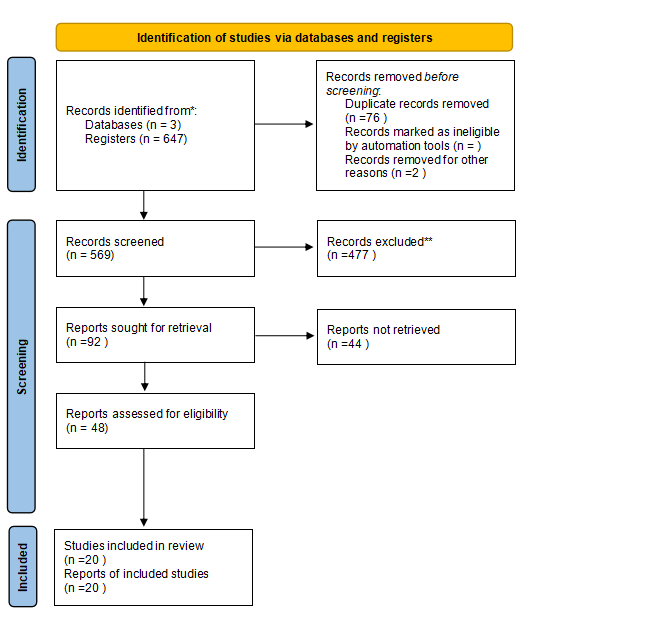
\includegraphics[width=0.8\linewidth]{figures/prisma.png}
    \caption{PRISMA flow diagram for new systematic reviews which included searches of databases and registers only }
    \label{fig:prisma}
\end{figure}

% Preamble (add once)
\newcolumntype{L}[1]{>{\raggedright\arraybackslash}p{#1}}

% Table
\begingroup
\footnotesize
\setlength{\tabcolsep}{4pt}
\renewcommand{\arraystretch}{1.05}
\begin{longtable}{@{}L{0.23\linewidth} L{0.57\linewidth} L{0.16\linewidth}@{}}

% --- Caption and label (must come first) ---
\caption{Studies included in the literature review.}
\label{tab:selectedArticles}\\

% --- Header (first page) ---
\toprule
\textbf{Ref.} & \textbf{Title} & \textbf{Thematic Area}\\
\midrule
\endfirsthead

% --- Header (next pages) ---
\multicolumn{3}{c}{{\tablename\ \thetable{} -- Continued from previous page}}\\
\toprule
\textbf{Ref.} & \textbf{Title} & \textbf{Thematic Area}\\
\midrule
\endhead

% --- Footer (all but last page) ---
\multicolumn{3}{r}{{\footnotesize\textit{Continued on next page}}}\\
\bottomrule
\endfoot

% --- Footer (last page) ---
% --- Footer (last page) ---
\bottomrule
\endlastfoot
~\parencite{ye_evolving_2025} & Evolving graph structure learning for multivariate time series forecasting & Dynamic Graph Structure Learning\\
~\parencite{gao_dynamic_2023} & Dynamic spatiotemporal interactive graph neural network for multivariate time series forecasting & Spatiotemporal GNN / MTS Forecasting\\
~\parencite{shang2021discretegraphstructurelearning} & DISCRETE GRAPH STRUCTURE LEARNING FOR FORECASTING MULTIPLE TIME SERIES & Discrete \& Regularized Graph Structure Learning\\
~\parencite{wu2020connectingdotsmultivariatetime} & Connecting the Dots: Multivariate Time Series Forecasting with Graph Neural Networks & Learned-Graph MTS Forecasting\\
~\parencite{xie2021dyhine} & Learning and Updating Node Embedding on Dynamic Heterogeneous Information Network & Dynamic Heterogeneous Graph Embedding\\
~\parencite{yilmaz2021demandgnn} & Enriching demand prediction with product relationship information using graph neural networks & Retail Demand Forecasting with GNNs\\
~\parencite{wang2022sparsificationfilteringspatialtemporalgnn} & Network Filtering of Spatial-temporal GNN for Multivariate Time-series Prediction & Graph Sparsification / Spatiotemporal GNN\\
~\parencite{wang2024hiercorrpool} & Multivariate Time-Series Representation Learning via Hierarchical Correlation Pooling Boosted Graph Neural Network & Relational Self-Supervised MTS Representation\\
~\parencite{jin2022generalizing} & On Generalizing Static Node Embedding to Dynamic Settings & Dynamic Graph Embedding\\
~\parencite{martirano2024dyhane} & DyHANE: dynamic heterogeneous attributed network embedding through experience node replay & Dynamic Heterogeneous Graph Embedding / Continual Learning\\
~\parencite{ma_graph_2021} & Graph Attention Networks with Positional Embeddings & Inductive Graph Neural Network Encoders\\
~\parencite{Hou2025PMEDGN} & Parallel multi-scale dynamic graph neural network for multivariate time series forecasting & Multi-scale Dynamic GNN / MTS Forecasting\\
~\parencite{10.1145/3534678.3539396} & Pre-training Enhanced Spatial-temporal Graph Neural Network for Multivariate Time Series Forecasting & Spatiotemporal GNN / Pre-training\\
~\parencite{WANG2024102429} & Contrastive learning enhanced by graph neural networks for Universal Multivariate Time Series Representation & Contrastive GNN / MTS Representation Learning\\
~\parencite{Yu20222362} & Regularized Graph Structure Learning with Semantic Knowledge for Multi-variates Time-Series Forecasting & Discrete \& Regularized Graph Structure Learning\\
~\parencite{liu_relational_2021} & Relational Time Series Forecasting for Retail Drugstores: A Graph Neural Network Approach & Retail Demand Forecasting with GNNs\\
~\parencite{MA2024123727} & Retail store-SKU level replenishment planning with attribute-space graph recurrent neural networks & Retail-Scale Learned-Graph Forecasting\\
~\parencite{der_matrix_2022} & Matrix Profile XXVII: A Novel Distance Measure for Comparing Long Time Series & Time Series Similarity \& Distance Metrics\\
~\parencite{kim2024stadgcn} & STAD-GCN: Spatial–Temporal Attention-based Dynamic Graph Convolutional Network for retail market price prediction & Dynamic Attention-Based Graphs in Retail\\
~\parencite{xu2024timegnn} & TimeGNN: Temporal Dynamic Graph Learning for Time Series Forecasting & Scalable Dynamic Graph Structure Learning\\
\end{longtable}
\endgroup




